\documentclass[12pt]{report}
\usepackage[utf8]{inputenc}
\usepackage{amsmath}
\usepackage{theorem}
\usepackage{geometry}
\usepackage{hyperref}
\usepackage{graphicx}
\usepackage{amsfonts}
\usepackage{enumitem}
\usepackage{algorithm}
\usepackage{algpseudocode}


\newtheorem{definition}{Definition}
\newtheorem{notation}{Notation}
\newtheorem{claim}{Claim}
\newtheorem{case}{Case}

\geometry{bottom=30mm, top=30mm, left=30mm, right=30mm}

\title{
    \textbf{\Huge{Theory Assignment 2}} \\
    \vspace*{15pt}
    \large{CSE222: \textit{Algorithm Design \& Analysis}}
}

\author{
    \href{mailto:divyajeet21529@iiitd.ac.in}{Divyajeet Singh (2021529)}
    \and
    \href{mailto:agamdeep21306@iiitd.ac.in}{Agamdeep Singh (2021306)}
}

\date{
    \vspace*{10pt}
    \textbf{\today}
}

\graphicspath{{./Assets/}}


\begin{document}
    \maketitle

    \section*{\huge{Problem-1}}
    The police department in the city of Computopia has made all the streets one-way.
    \begin{enumerate}[label=(\alph*)]
        \item
        The mayor of the city claims that it is possible to legally drive from an intersection to any other intersection.
        Formulate this problem as a graph theoretic problem and explain why it can be solved in linear time.
        \item
        Suppose the mayor's claim was found to be wrong. She has now made a weaker claim:
        \textit{"If you start driving from the town-hall, navigating one-way streets, then no matter where you reach,
        there is always a way to drive legally back to the town-hall."}
        Formulate this weaker property as a graph theoretic problem and explain how it can be solved in linear time.
    \end{enumerate}

    \subsection*{Input}
    A directed graph $G = (V, E)$ representing the layout of the city.
    $V$ is the set of all intersections and $E$ is the set of all one-way streets in Computopia.
    \vspace*{7.5pt} \\
    \textbf{Note:} \textit{Formulation of the problem as a graph theoretic problem is given in the subsequent subsection.}

    \subsection*{Output}
    \begin{enumerate}[label=(\textbf{\alph*})]
        \item A boolean value \textsc{True} if the mayor's claim holds, else \textsc{False}.
        \item A boolean value \textsc{True} the mayor's weaker claim holds, and \textsc{False} otherwise.
    \end{enumerate}

    \subsection*{Solution}
    The two sub-parts of the given problem can both be solved in linear time using the concept of strongly connected components in a directed graph.
    By definition, a component of a graph $G$ is strongly connected if there exists a path from every vertex in the component to every other vertex in the component.
    The following sections discuss approaches to solving the two sub-problems in detail.

    \subsubsection*{Formulation as a graph theoretic problem}
    Since the given problem deals with the layout of a city, it can be naturally solved using graphs.
    Each intersection in the city can be considered as a vertex, $v \in V$, and each one-way street as a directed edge, $(u \to v) \in E$, where $u, v \in V$.
    One-way streets naturally represent directed edges as both can only be traversed in one direction. \\
    In this manner we create a graph $G = (V, E)$ based on the city's layout.
    \footnote{For \textbf{Problem 1 (b)}, we assume that the town-hall is located at an intersection, $v_{t} \in V$.}

    \subsection*{Problem 1 (a)}
    \subsubsection*{The Solution Description}
    This sub-part can be solved in linear time using the popular Kosaraju's Algorithm
    \footnote{
        Kosaraju's Algorithm was disucssed in Lecture-12 of the course \textbf{CSE222} by \href{mailto:debarka@iiitd.ac.in}{Dr Debarka Sengupta}, Winter 2023.
    } to find strongly connected components in a directed graph.
    According to the mayor's claim, we must be able to legally drive from any intersection from any other intersection in the city.
    This can be achieved if and only if there exists a path between every pair of vertices in $G$.
    This, by defintion, is equivalent to $G$ being strongly connected. \\
    Hence, the mayor's claim would be considered true if and only if $G$ contains exactly one stronly connected component that contains all vertices $v \in V$.

    \subsubsection*{The complete Algorithm and Pseudocode}
    The complete algorithm consists of the following steps:
    \begin{enumerate}
        \item
        Use Kosaraju's Algorithm to find all the strongly connected components of $G$.
        The algorithm makes use of a DFS traversal on $G$ and $G^{T}$, the transposed graph of $G$.
        \item Determine if there is exactly one strongly connected component, say $S$, and if $S$ contains all vertices $v \in V$.
    \end{enumerate}
    The pseudocode for the complete algorithm is given in Algorithm~(\ref{alg:claim-check}).

    \begin{algorithm}
        \caption{An algorithm to check the mayor's stronger claim}
        \label{alg:claim-check}
        \begin{algorithmic}[1]
            \Procedure{Check-claim}{$G = (V, E)$}
            \State $C \gets \Call{Kosaraju-algorithm}{G}$ \Comment{Returns a list of all SCCs in $G$}
            \If{$|C| = 1$ \textbf{and} $|V| = |C[0]|$}
                \State \Return \textsc{True}
            \Else
                \State \Return \textsc{False}
            \EndIf
            \EndProcedure
        \end{algorithmic}
    \end{algorithm}

    \subsubsection*{Runtime Analysis of the Algorithm}
    The algorithm determines the fallacy of the mayor's claim in linear time with respect to the number of intersections and one-way streets in the city. \\
    It makes use of Kosaraju's Algorithm, which finds all SCCs in a graph in $O(|V|+|E|)$ time.
    \vspace*{10pt} \\
    Hence, dominated by the time complexity of Kosaraju's Algorithm, the time complexity of the algorithm is $O(|V|+|E|)$.

    \subsubsection*{Proof of Correctness}
    It can be proven that the algorithm correctly determines if one can legally drive to any intersection from any other intersection.
    According to the mayor's claim, there must exist a path from every intersection to every other intersection.
    Hence, the following cases may arise:
    \begin{enumerate}
        \item
        If $G$ contains more than one SCC, then there exists a vertex $v \in V$ such that $v$ is not reachable from some vertex $u \in V$.
        Hence, the mayor's claim is false.
        \item
        If $G$ contains exactly one SCC, but the SCC does not contain all vertices in $V$, then the mayor's claim is false.
        In this case, there exists a vertex $v \in V$ such that $v$ is not reachable from any other vertex in $G$.
        \item
        If $G$ contains exactly one SCC containing all vertices in $V$, then the mayor's claim is true.
        In this case, there exists a path from every vertex in $G$ to every other vertex in $G$.
    \end{enumerate}
    The algorithm handles all the above cases, and hence correctly determines the fallacy of the mayor's claim.

    \subsection*{Problem 1 (b)}
    \textbf{Assumption:} The town-hall is located at an intersection in Computopia.

    \subsubsection*{The Solution Description}
    This sub-part can be solved in linear time by using Kosaraju's algorithm again.
    However, in this case, we must check if the town-hall is a part of a strongly component in $G$. \\
    According to the mayor's weaker claim, all intersections reachable from the town-hall have at least one way to legally drive back to the town-hall.
    This can be achieved if an only if the town-hall is a part of a strongly connected component in $G$. \\
    Hence, the mayor's weaker claim would be considered true if and only if the town-hall is a part of a strongly connected component in $G$.

    \subsubsection*{The complete Algorithm and Pseudocode}
    The complete algorithm consists of the following steps:
    \begin{enumerate}
        \item
        Use Kosaraju's Algorithm to find all the strongly connected components of $G$.
        The algorithm makes use of a DFS traversal on $G$ and $G^{T}$, the transposed graph of $G$.
        \item Determine if the town-hall is a part of a strongly connected component in $G$.
    \end{enumerate}
    The pseudocode for the complete algorithm is given in Algorithm~(\ref{alg:check-weak-claim}).

    \begin{algorithm}
        \caption{An algorithm to check the mayor's weaker claim}
        \label{alg:check-weak-claim}
        \begin{algorithmic}[1]
            \Procedure{Check-claim}{$G = (V, E), v_{t}$}
            \State $C \gets \Call{Kosaraju-algorithm}{G}$ \Comment{Returns a list of all SCCs in $G$}
            \For{$i \gets 1$ \textbf{to} $|C|$}
                \If{$v_{t} \in C[i]$}
                    \State \Return \textsc{True}
                \EndIf
            \EndFor
            \State \Return \textsc{False}
            \EndProcedure
        \end{algorithmic}
    \end{algorithm}

    \subsubsection*{Runtime Analysis of the Algorithm}
    The algorithm determines the fallacy of the mayor's claim in linear time with respect to the number of intersections and one-way streets in the city. \\
    It again makes use of the $O(|V|+|E|)$ time Kosaraju's Algorithm.
    The subsequent checking of whether the town-hall $v_{t}$ is a part of any of the SCCs takes at max $|V|$ operations.
    This is because the total number of vertices in all the components combined is, at max, $|V|$.
    \vspace*{10pt} \\
    Hence, dominated by the time complexity of Kosaraju's Algorithm, the time complexity of the algorithm is $O(|V|+|E|)$.

    \subsubsection*{Proof of Correctness}
    It can be proven that the algorithm correctly determines if the mayor's weaker claim is true.
    According to the mayor's weaker claim, an intersection reachable from the town-hall must have at least one way to legally drive back to the town-hall.
    Hence, the following cases may arise:
    \begin{enumerate}
        \item
        If the town-hall $v_{t}$ is not a part of any of the SCCs, then the mayor's weaker claim is false.
        In this case, there exists some vertex $v \in V$ such that $v$ is reachable from the town-hall, but there is no way to legally drive back to the town-hall from $v$.
        \item
        If the town-hall $v_{t}$ is a part of a SCC, then the mayor's weaker claim is true.
        By definition, a SCC contains all vertices that are reachable from each other.
        Hence, there exists a path from every intersection reachable from the town-hall back to the town-hall.
    \end{enumerate}
    The algorithm handles all the above cases, and hence correctly determines the fallacy of the mayor's weaker claim.

    \pagebreak

    \section*{\huge{Problem-2}}
    Assume that $n$ is the number of vertices in a graph.
    Then, given an edge-weighted connected undirected graph $G = (V, E)$ with $n + 20$ edges, design an algorithm that runs in $O(n)$
    time and outputs an edge with the smallest weight, connected in a cycle of $G$.
    You must give a justification why your algorithm works correctly.

    \subsection*{Input}
    An edge-weighted connected undirected graph $G = (V, E)$ such that $|V| = n$ and $|E| = n + 20$.

    \subsection*{Output}
    An edge $(v, w)$ with the smallest weight, connected in a cycle of $G$.

    \subsection*{Solution}
    The given problem can be solved in $O(n)$ time using the concept of cut-edges.
    We make use of the fact that cut-edges, by definition, are not included in any cycle in a graph, and all non-cut-edges are included in some cycle.
    Hence, we can find the edge with the smallest weight in $G$ that is not a cut-edge.

    \subsubsection*{Terminologies and Definitions}
    \begin{definition}[Cut-Edge]
        \label{def:cut-edge}
        An edge $(v, w) \in E$ is a cut-edge if removing it from the graph $G = (V, E)$ increases the number of connected components in $G$.
        For a connected graph $G$, removal of a cut-edge disconnects $G$.
    \end{definition}

    \begin{figure}[htp]
        \begin{center}
            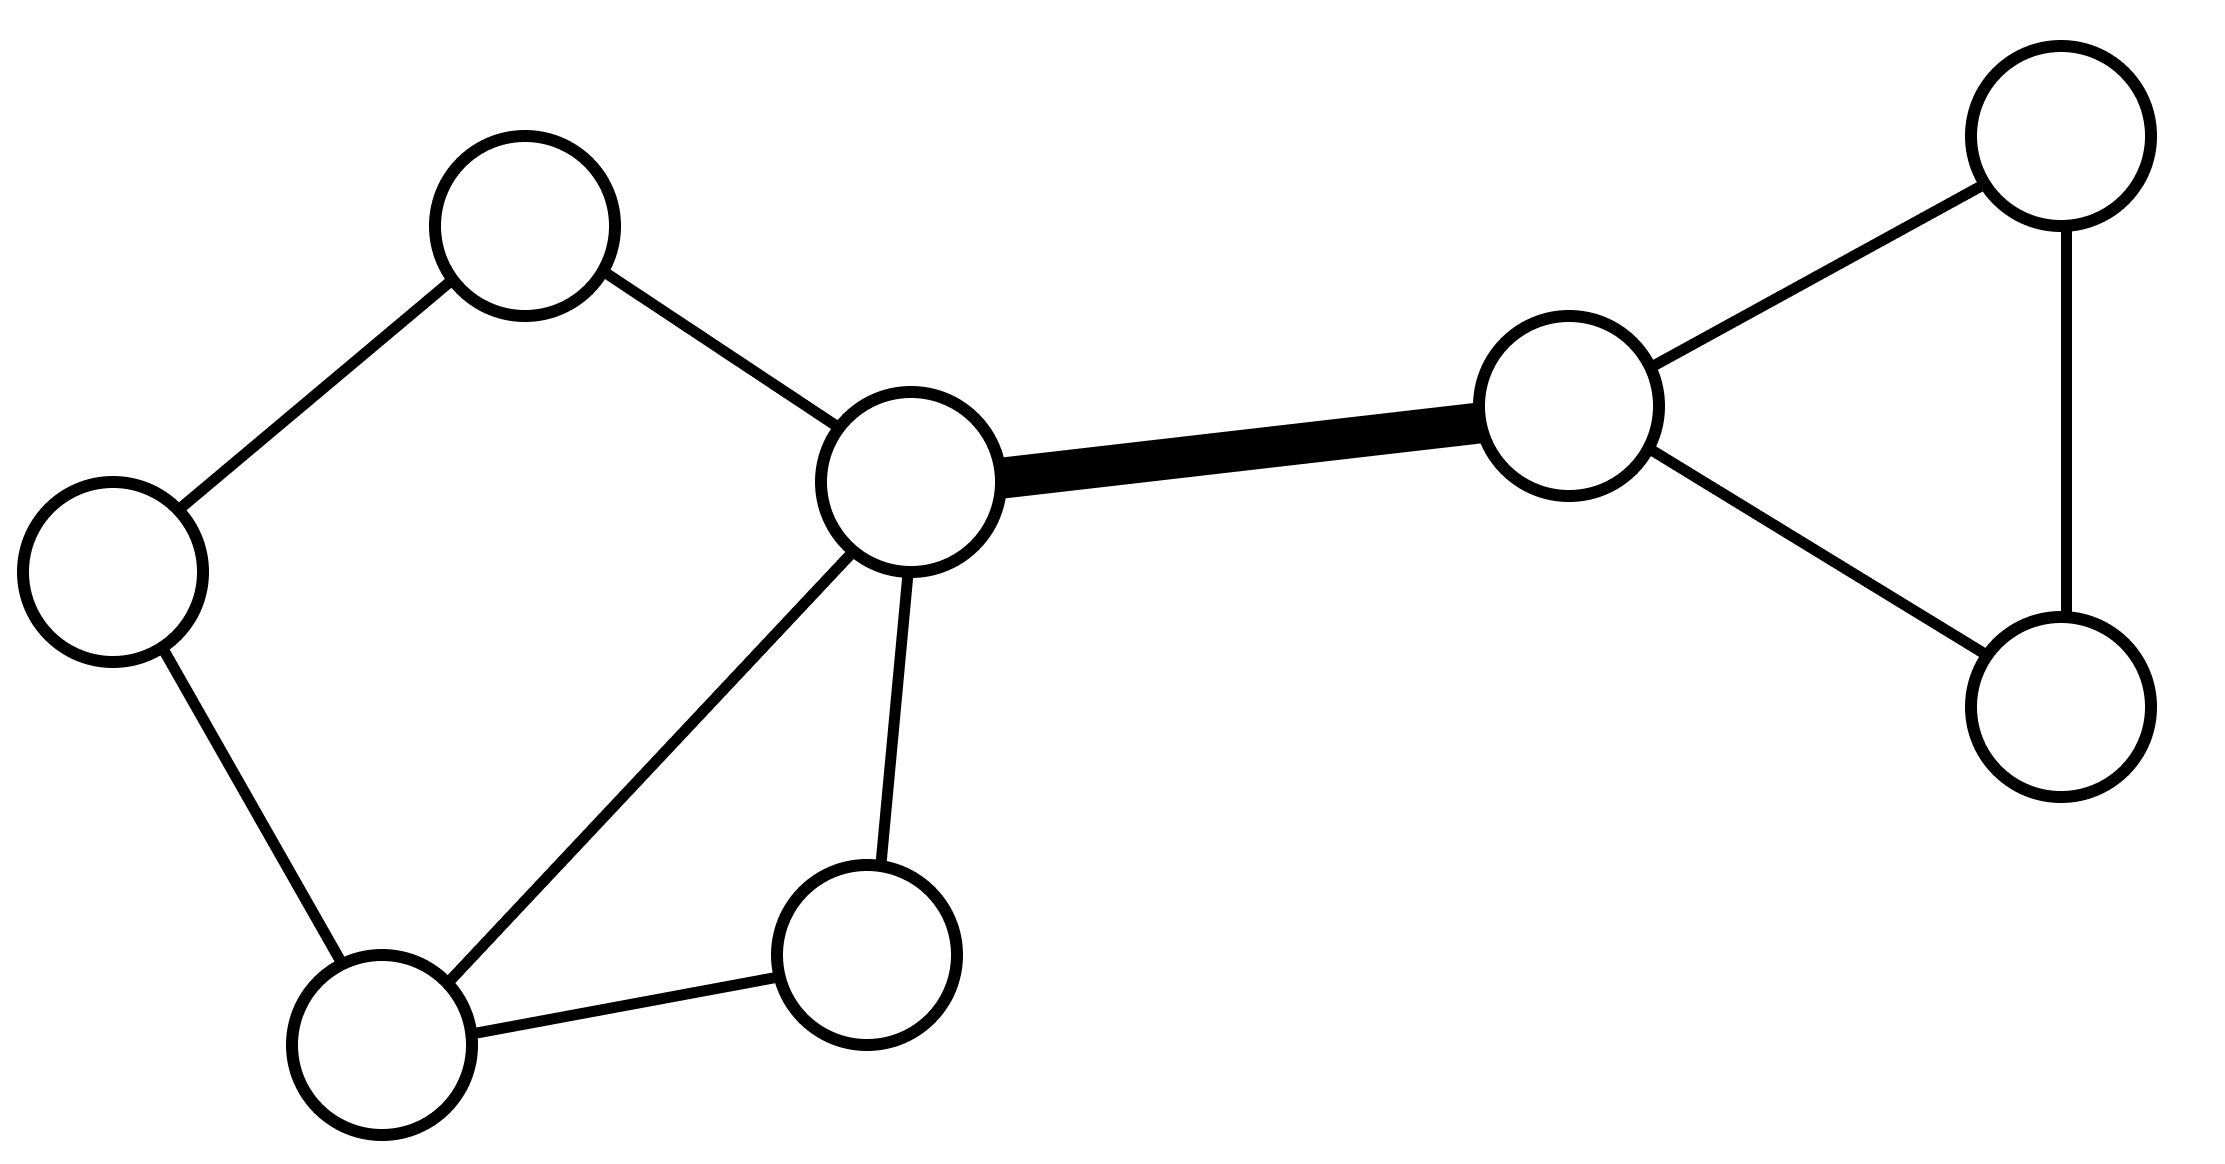
\includegraphics[width=0.65\textwidth]{cut-edge.png}
        \end{center}
        \caption{The thick edge is a cut-edge (removing it creates two connected components)}
        \label{fig:cut-edge}
    \end{figure}

    \subsubsection*{The Solution Description}
    The solution simply involves finding and marking the cut-edges in $G$.
    Once all edges are marked, we can find the edge with the smallest weight in $G$ that is not marked by iterating over $E$.

    \begin{claim}
        An edge $(v, w) \in E$ is a cut-edge if it is not included in any cycle of $G$.
    \end{claim}
    \textit{Proof.}
    \begin{quote}
        $\Rightarrow$ (If $(v, w) \in E$ is a cut-edge, then it is not included in any cycle in $G$.) \\
        We prove the contrapositive of the claim. \\
        Let $e = (v, w) \in E$ be involved in a cycle. Then, there exists a path from $v$ to $w$ in $G$
        that does not contain $e$, and hence, removing $e$ from $G$ does not disconnect $G$.
        So, $e$ is not a cut-edge. \\
        By contraposition, the forward implication is proved.
        \vspace*{7.5pt} \\
        $\Leftarrow$ (If $(v, w) \in E$ is not included in any cycle in $G$, then it is a cut-edge.) \\
        We prove the contrapositive of the claim. \\
        Let $e = (v, w) \in E$ be a non-cut-edge. Then, we can safely remove $e$ from $G$ and still have a connected graph,
        i.e., there still exists a path from $v$ to $w$ in $G$.
        So $e$ must be included in some cycle. \\
        By contraposition, the backward implication is proved.
        \vspace*{7.5pt} \\
        Hence, the claim is proved. \hfill $\square$
    \end{quote}
    The above claim is the key to solving the problem in linear time, as the cut-edges can be identified in $G$ in $O(|V|+|E|)$ time.

    \subsubsection*{The complete Algorithm}
    The complete algorithm consists of the following steps:
    \begin{enumerate}
        \item Identify all the cut-edges and mark them.
        \item Find the edge with the smallest weight in $E$ that is not marked.
    \end{enumerate}

    \subsubsection*{Pseudocode for the Find-cut-edges subroutine}
    To find the cut-edges of $G$, we use a subroutine $\Call{Find-cut-edges}{G}$.
    The subroutine uses a DFS traversal on the input graph $G = (V, E)$ and returns a hash table $C$ of edges, in which
    $C[e] = 1$ if and only if $e$ is a cut-edge.
    \vspace*{10pt} \\
    The algorithm uses a DFS traversal on the graph, while maintaining the following data structures:
    \begin{enumerate}
        \item $M[v \in V]$: To keep track of visited vertices.
        \item $T_{in}[v \in V]$: To store the time at which a vertex is first visited.
        \item $T_{low}[v \in V]$: To store the lowest time of discovery of all vertices reachable from $v$.
        \item $C[e \in E]$: A hash table to mark the cut-edges.
    \end{enumerate}
    The main idea behind the algorithm is to correctly track and update the discovery times of each vertex $v$ and the lowest discovery time of all its ancestors.
    \vspace*{10pt} \\
    This ensures that if $T_{low}[w] > T_{in}[v]$, then $w$ cannot be reached from any of the ancestors of $v$.
    If $w$ was reachable from any of the ancestors of $v$, then $T_{low}[w] \leq T_{in}[v]$, i.e. it would have already been visited,
    in which case, $T_{low}[v]$ is updated to $T_{in}[w]$ if it's less than $T_{low}[v]$. \\
    So, $(v, w) \in E$ cannot be a part of a cycle, and hence, must be a cut-edge.
    \footnote{
        A formal proof of correctness of this subroutine is given in the section \textbf{Proof of Correctness}.
    }
    \vspace*{10pt} \\
    The pseudocode for the subroutine implemented using Tarjan's Algorithm is given in Algorithm~(\ref{alg:cut-edges}).
    \footnote{
        The subroutine assumes that the graph $G$ is connected and does not contain any self-loops.
    }

    \begin{algorithm}
        \caption{Tarjan's Algorithm to mark the cut-edges in a connected graph $G$}
        \label{alg:cut-edges}
        \begin{algorithmic}[1]
            \Procedure{Mark-cut-edges}{$G = (V, E)$}:
                \State $M[v \in V] = T_{in}[v \in V] = T_{low}[v \in V] \gets 0$
                \State $C[e \in E] \gets 0$
                \State $t \gets 0$
                \Procedure{Dfs}{$v$, $p$}:
                    \State $M[v] \gets 1$
                    \State $T_{in}[v] = T_{low}[v] \gets t$
                    \State $t \gets t + 1$
                    \For{$(v, w) \in E$}
                        \If{$w = p$}
                            \State \textbf{continue}
                        \ElsIf{$M[w] = 0$}
                            \State $\Call{Dfs}{w, v}$
                            \State $T_{low}[v] \gets \min{\{T_{low}[v], T_{low}[w]\}}$
                            \If{$T_{low}[w] > T_{in}[v]$}
                                \State $C[(v, w)] \gets 1$
                            \EndIf
                        \Else
                            \State $T_{low}[v] \gets \min{\{T_{low}[v], T_{in}[w]\}}$
                        \EndIf
                    \EndFor
                \EndProcedure
                \State $\Call{Dfs}{v_{0}, v_{0}}$ \Comment{$v_{0}$ is any arbitrary vertex in $V$}
                \State \Return $C$
            \EndProcedure
        \end{algorithmic}
    \end{algorithm}

    \subsubsection*{Pseudocode for the complete algorithm}
    The pseudocode for the complete algorithm is given in Algorithm~(\ref{alg:cycle-edge}).

    \begin{algorithm}
        \caption{An algorithm to find the least weight edge connected in a cycle of $G$}
        \label{alg:cycle-edge}
        \begin{algorithmic}[1]
            \Procedure{Cycle-edge}{$G = (V, E)$}:
                \State $C \gets \Call{Mark-cut-edges}{G}$
                \State $e_{min}.weight \gets \infty$
                \For{$e \in E$}
                    \If{$C[e] = 0$}
                        \If{$e.weight < e_{min}.weight$}
                            \State $e_{min} \gets e$
                        \EndIf
                    \EndIf
                \EndFor
                \State \Return $e_{min}$
            \EndProcedure
        \end{algorithmic}
    \end{algorithm}

    \subsubsection*{Runtime Analysis of the Algorithm}
    The algorithm makes use of the $\Call{Mark-cut-edges}{G}$ subroutine, which runs in $O(|V|+|E|)$ time.
    This is because the subroutine only implements a modified DFS traversal on the graph, with modifications like
    array lookups and hash table insertions. Since both of these operations take constant time, the total time
    taken by the subroutine is $O(|V|+|E|)$.
    \vspace*{10pt} \\
    The main algorithm also runs in $O(|V|+|E|)$ time, since it only makes a single call to the subroutine
    and the subsequent step iterates over the edge-set $E$ while maintaining a minimum edge $e_{min}$, which takes $\Theta(|E|)$ time.
    \vspace*{10pt} \\
    Hence, the total time taken by the algorithm is $O(|V|+|E|)$. \\
    Since we're given $|V| = n$ and $|E| = n + 20$, the overall time complexity of the algorithm is $O(n)$.

    \vfill

    \subsubsection*{Proof of Correctness}
    The correctness of the algorithm can be proved by a series of the following claims.

    \begin{claim}
        The subroutine correctly identifies all cut-edges in the graph $G$.
    \end{claim}
    \textit{Proof.}
    \begin{quote}
        Suppose $(v, w)$ is a cut-edge in $G$. \\
        By definition, $w$ cannot be reached from any of the ancestors of $v$.
        So, $T_{in}[w]$, the discovery time of $w$, which is equal to $T_{low}[w]$ as it has not been explored yet,
        must be greater than $T_{in}[v]$, the discovery time of $v$.
        All such edges are marked by the subroutine. \\
        Hence, the claim is proved. \hfill $\square$
    \end{quote}

    \begin{claim}
        \label{claim:non-cut-edge}
        The subroutine does not mark any non-cut-edge in the graph $G$.
    \end{claim}
    \textit{Proof.}
    \begin{quote}
        Suppose $(v, w)$ is a non-cut-edge in $G$. \\
        By definition, $w$ can be reached from some ancestor of $v$.
        So, $T_{low}[w]$, the lowest time of discovery of the vertices reachable from $w$,
        must be at most equal to $T_{in}[v]$, the discovery time of $v$.
        This is because $T_{low}[w]$ must have been relaxed to $T_{in}[v]$ at some point in the DFS traversal due to presence of a cycle.
        Hence, the edge $(v, w)$ is not marked by the subroutine. \\
        Hence, the claim is proved. \hfill $\square$
    \end{quote}

    \begin{claim}
        The algorithm correctly identifies the least weight edge connected in a cycle of $G$.
    \end{claim}
    \textit{Proof.}
    \begin{quote}
        Suppose $e_{min}$ is the least weight edge connected in a cycle of $G$. \\
        By definition, $e_{min}$ is not a cut-edge.
        By Claim~(\ref{claim:non-cut-edge}), $e_{min}$ must not be marked.
        Finding the least weight edge among the non-marked edges, hence, identifies the least weight edge connected in a cycle of $G$. \\
        Hence, the claim is proved. \hfill $\square$
    \end{quote}

    \pagebreak

    \section*{\huge{Problem3}}
    Suppose that $G$ is a directed acyclic graph with the following features:
    \begin{itemize}
        \item $G$ has a single source $s$ and several sinks $t_{1}, t_{2}, \dots, t_{k}$.
        \item Each edge $(v \to w)$ (i.e. an edge directed from $v$ to $w$) has an associated weight $P[v \to w]$ between $0$ and $1$.
        \item For each non-sink vertex $v$, the total weight of all the edges leaving $v$ is $1$, i.e.
        \begin{equation}
            \label{eq:total_weight}
            \sum_{(v \to w) \in E} P[v \to w] = 1
        \end{equation}
    \end{itemize}
    The weights $P[v \to w]$ define a random walk in $G$ from $s$ to some sink $t_{i}$.
    After reaching any non-sink vertex $v$, the walk follows the edge $(v \to w)$ with probability $P[v \to w]$.
    All the probabilities are mutually independent. \\
    Describe and analyze an algorithm to compute the probability that this random walk reaches sink
    $t_{i} \ \forall \ i \in \{ 1, 2, \dots, k \}$. \\
    An example of such a graph is shown in Figure~(\ref{fig:dag}).
    \footnote{The weights are not shown for simplicity.}

    \begin{figure}[htp]
        \begin{center}
            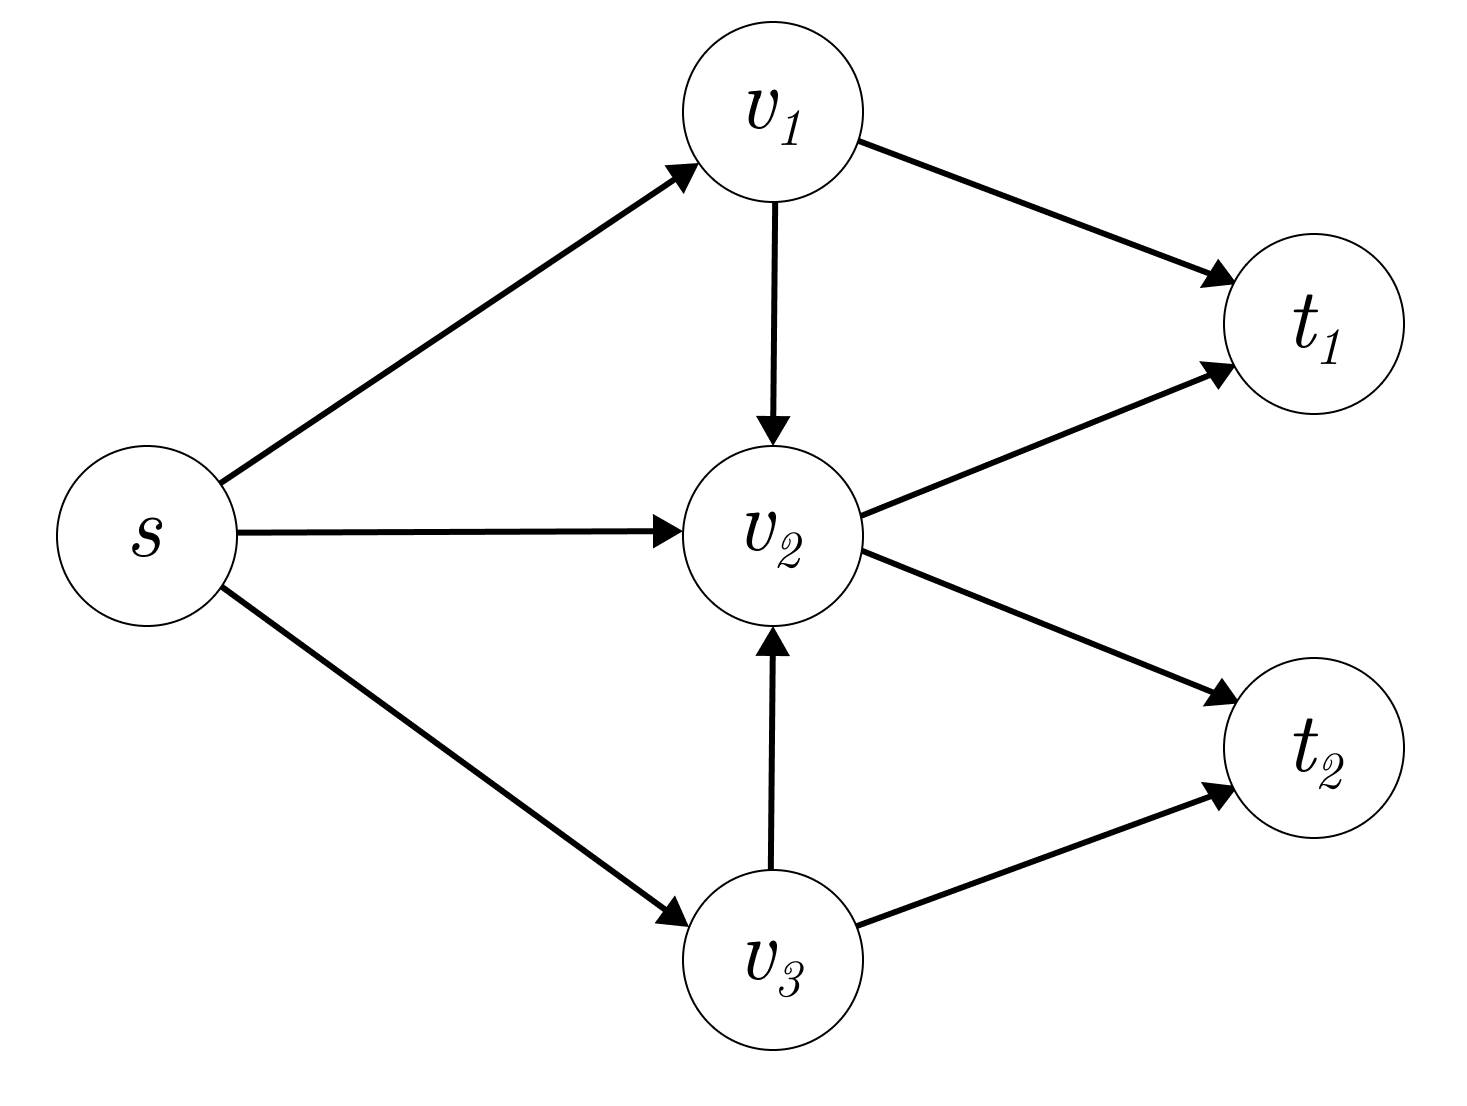
\includegraphics[width=0.45\textwidth]{dag.png}
        \end{center}
        \caption{A directed acyclic graph with a single source and several sinks.}
        \label{fig:dag}
    \end{figure}

    \subsection*{Input}
    A weighted directed acyclic graph $G = (V, E)$ having the above properties.

    \subsection*{Output}
    A sequence of probabilities $P[t_{1}], P[t_{2}], \dots, P[t_{k}]$, where $P[t_{i}]$ is the probability that the random walk
    reaches sink $t_{i} \ \forall \ i \in \{ 1, 2, \dots, k \}$.

    \subsection*{Solution}
    The given problem can be efficiently solved by applying dynamic programming on the topologically sorted graph $G$.
    It allows for the calculation of the probability of reaching every edge $v \in V$ starting from $s$.

    \subsubsection*{Notations Used}
    \begin{notation}[$P{[v \to w]}$]
        The weight of the edge $(v \to w) \in E$. This is also the probability of following the edge $(v \to w)$ for the random walk from $v$.
    \end{notation}

    \begin{notation}[$P{[v]}$]
        The total probability of reaching vertex $v$ from the source $s$.
        It also denotes the entry for vertex $v$ in the dynamic programming table.
    \end{notation}

    \subsubsection*{Preprocessing}
    We first obtain a total ordering of the given graph $G$ by topologically sorting it.
    This can be done using the $\Call{Topological-sort}{G}$ routine covered in class. \\
    The sorting step can be achieved in $\Theta(|V|+|E|)$ time. \\
    \vspace*{2.5pt} \\
    \textit{Reason for Sorting:}
    \vspace*{2.5pt} \\
    When $G$ is sorted in the aforementioned fashion, then the vertices are ordered such that $v$ appears before $w$ if $(v \to w) \in E$.
    This allows us to calculate $P[w]$ by using the probabilities $P[v] \ \forall \ (v \to w) \in E$.
    This is possible because of equation \eqref{eq:total_weight} and the fact that the probabilities are mutually independent.

    \begin{figure}[htp]
        \begin{center}
            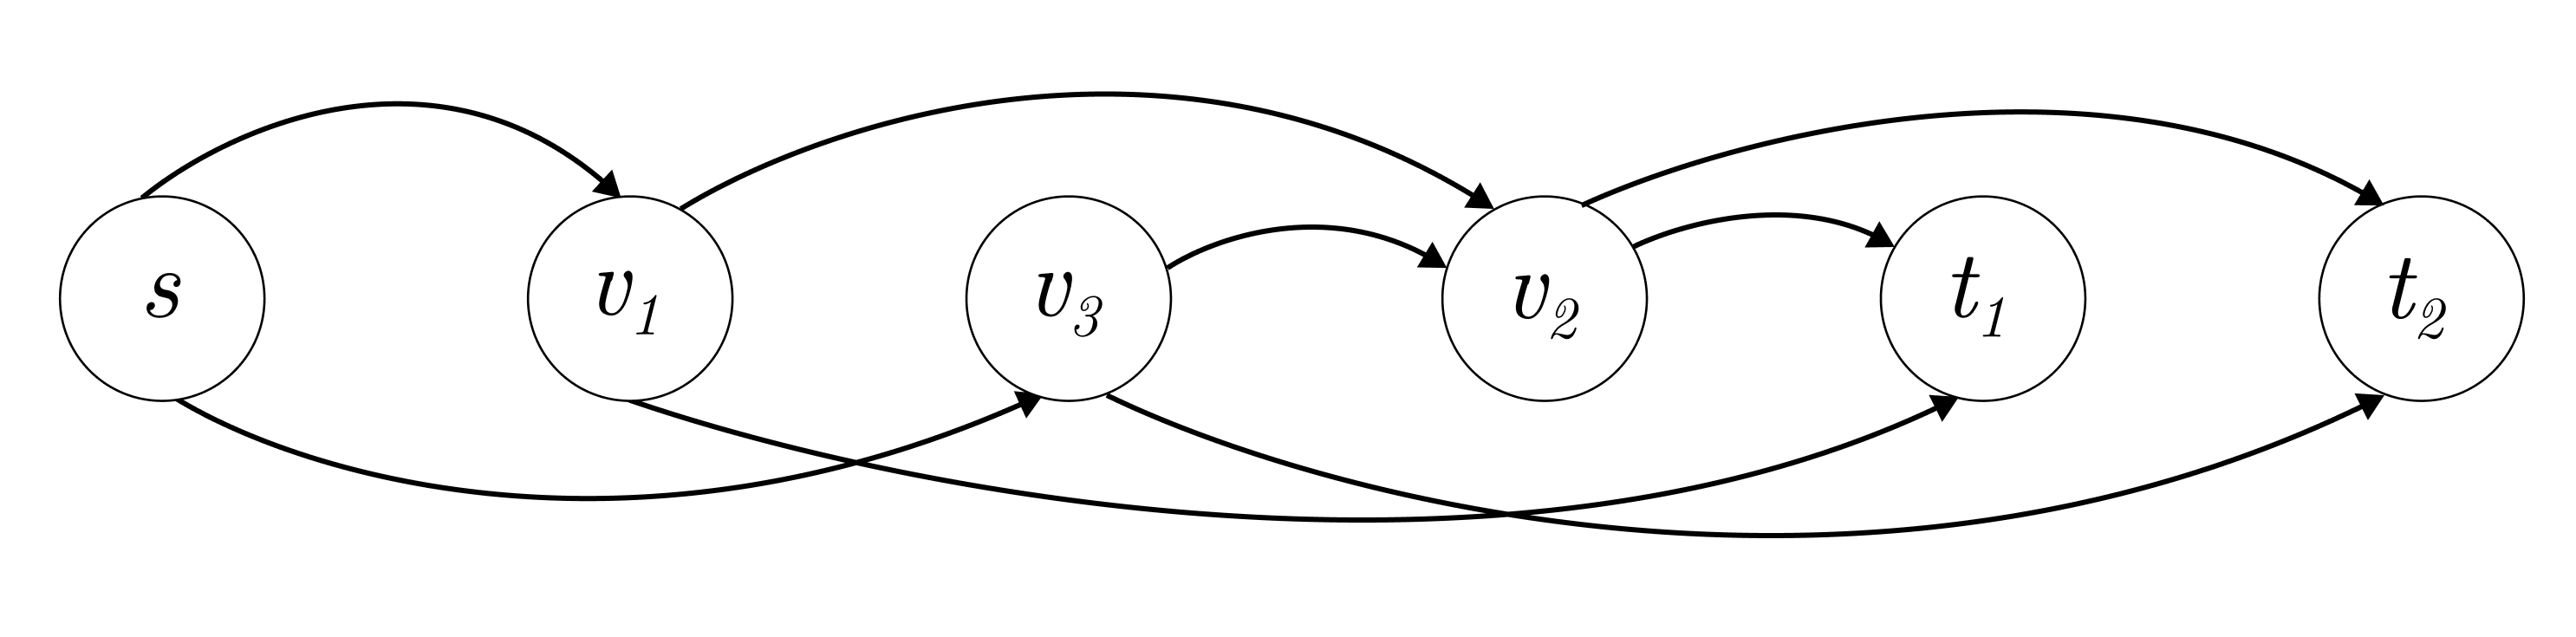
\includegraphics[width=0.75\textwidth]{top-sort.png}
        \end{center}
        \caption{A topologically sorted version of the graph in Figure~(\ref{fig:dag}).}
        \label{fig:top-sort}
    \end{figure}

    \subsubsection*{Decomposition into Sub-Problems}
    The given problem of finding $P[t_{i}] \ \forall \ 1 \leq i \leq k$ is broken down into overlapping sub-problems of the form $P[v]$, where $v$ is not a sink.
    For each problem $P[v]$, we intend to find the probability of reaching $v$ from $s$. \\
    Each probability $P[v]$ can be found by adding the probabilities of reaching $v$ from all vertices having an edge directed to $v$.
    The existence of $P[u] \ \forall \ (u \to v) \in E$ is guaranteed by the topological ordering. \\
    Hence, this decomposition of the given problem into smaller sub-problems guarantees substructure optimalilty.
    This is because at any step, we can find the optimal solution using the optimzal solutions obtained in the previous steps.

    \subsubsection*{Recurrence Relation}
    Let $P[v]$ be the total probability of reaching any vertex $v$ from the source $s$.
    Then, the following recurrence relation can be defined:
    \begin{equation}
        P[v] = \begin{cases}
            1 & \text{if } v = s \\
            \sum\limits_{(u \to v) \in E} P[u] \times P[u \to v] & \text{otherwise}
        \end{cases}
    \end{equation}
    Using the above recurrence relation, we can find $P[v] \ \forall \ v \in V$ and maintain it in a $|V| \times 1$ dynamic programming table.

    \subsubsection*{Base Case and Solvable Sub-Problems}
    The base case for the above recurrence relation is $P[s] = 1$.
    This is because the probability of reaching $s$ from the source is $1$, as the random walk starts from $s$.
    \vspace*{10pt} \\
    The sub-problems that solve the original problem are $P[t_{i}] \ \forall \ 1 \leq i \leq k$, the probabilities of reaching the sinks $t_{i}$ from $s$.

    \subsubsection*{The complete Algorithm and Pseudocode}
    The complete algorithm consists of the following steps:
    \begin{enumerate}
        \item Topologically sort the graph $G$ to get a total ordering of $V$.
        \item Initialize the dynamic programming table $P$ following the base case.
        \item Iterate over the vertices in their topological order and tabulate $P$ using the above recurrence relation.
        \item Return $P[t_{1}], P[t_{2}], \dots, P[t_{k}]$, the total probabilities of reaching the sinks from $s$.
    \end{enumerate}
    The pseudocode for the complete algorithm is given in Algorithm~(\ref{alg:sink-prob}).
    \footnote{
        The pseudocode of the algorithm makes use of notations introduced in the section \textbf{Notations Used}.
        Here, $P[v \in V_{T}]$ denotes a $|V_{T}| \times 1$ table ordered in the same way as $V_{T}$.
    }

    \begin{algorithm}
        \caption{An algorithm to find the probabilities of reaching the sinks from $s$}
        \label{alg:sink-prob}
        \begin{algorithmic}[1]
            \Procedure{Sink-probability}{$G = (V, E)$}:
                \State $V_{T} = \Call{Topological-sort}{G}$
                \State $P[v \in V_{T}] \gets 0$
                \State $P[s] \gets 1$
                \For{$v \in V_{T}$}
                    \For {$(u \to v) \in E$}
                        \State $P[v] \gets P[v] + P[u] \times P[u \to v]$
                    \EndFor
                \EndFor
                \State \Return $P[t_{1}], P[t_{2}], \dots, P[t_{k}]$
            \EndProcedure
        \end{algorithmic}
    \end{algorithm}

    \vfill

    \subsubsection*{Runtime Analysis of the Algorithm}
    The following operations are performed in the algorithm:
    \begin{enumerate}
        \item $\Call{Topological-sort}{G}$: This step takes $\Theta(|V|+|E|)$ time.
        \item Initialization of the dynamic programming table $P$, which takes $\Theta(|V|)$ time.
        \item The dynamic programming step takes $\Theta(|V|+|E|)$ time, as it iterates over all vertices,
        while accessing the edges incident on each vertex.
        Analogous to a BFS traversal, the total number of iterations of the outer loop is $|V|$ and the inner loop is $|E|$.
    \end{enumerate}
    Dominated by the sorting step and the dynamic programming step, the time complexity of the algorithm is $\Theta(|V|+|E|)$.
    \vfill
    \pagebreak

    \section*{Bibliography}
    \begin{enumerate}
        \item
        \href{
            https://iq.opengenus.org/find-cut-edges-in-a-graph/#:~:text=A%20cut%20edge%20e%20%3D%20uv,belong%20to%20the%20DFS%20tree.
            }{\textbf{OpenGenius IQ:} Tarjan's Algorithm to find cut-edges in a Graph}
        \item
        \href{
            http://web.math.ucsb.edu/~padraic/ucsb_2013_14/math137a_w2014/math137a_w2014_lecture3.pdf
        }{\textbf{USCB Math137A: (Lemma 1}) Cut-edges are not contained in cycles}
    \end{enumerate}

\end{document}